\chapter{Лекция 1. Введение}

\section{Список литературы}

Потом допишем

\section{Введение}

\subsection{Взаимодействие ядра и прикладных программ}

Основной интерфейс взаимодействия ядра и прикладных программ использует системные вызовы. Системные вызовы не являются обычными
функциями и как правило реализуются на основе программных прерываний (те кто программировал на языке ассемблера, например, под DOS,
наверняка помнят инструкции вида int 20h).

\paragraph{Почему так?.} Существует жесткое разделение между kernel и user space, процессы прикладных программ полагаются на то,
что им доступна вся память и вся аппаратура, кроме того, ничего не подозревают о других процессах (условно), в ядре же все не так,
и требуется переходить из одного режима процессора в другой, т. е. изменять привелегии выполнения кода.

Что же можно сказать о прерываниях? Каждое прерывание идентифицируется некоторым номером, программные прерывания могут маскироваться
(в самом простом случае этому состоянию просто соответсвует флаг в регистре состояния), т. е. обработка прерываний (не всех, например,
прерывание при делении на 0) может быть запрещена. 

Обраточики прерываний почти обычные программы, которые часто разделяются на 2 части - верхнюю и нижнюю половины. В чем смысл такого
разделения? Ответ прост, ядро может одновременно выполнять только один обработчик прерывания, при этом никакие другие задачи не
выполняются, поэтому желательно, чтобы обработчики выполнялись как можно быстрее. Поэтому критически необходимые действия выполняются
в верхней половине, в ней же происходит планирование выполнения нижней половины, которая исполняется уже отложенно, не в контексте
прерывания, диспетчиризируется почти как обычный процесс.

\subsection{Структура ОС и выполняемые задачи}

\begin{figure}
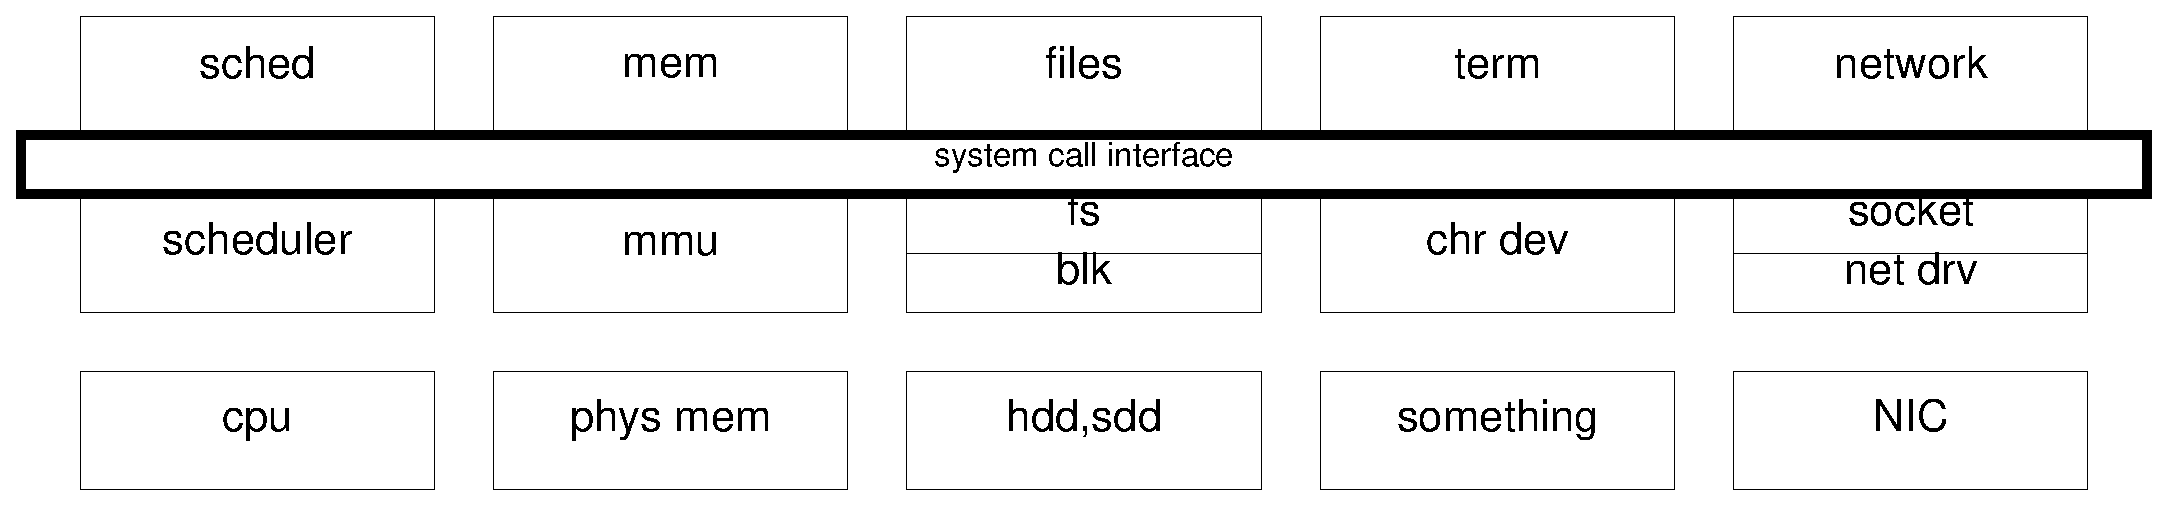
\includegraphics[width=\linewidth]{os_arch}
\caption{Основные блоки ОС}
\label{img::les1::os_arch}
\end{figure}

Принято разделять ядра ОС на два основных блока: монолитные и микроядерные. Монолит воплощает концепцию все в себе, т. е. все
механизмы ядра заключены в одном бинарнике, в отличие от микроядра, которое включает в себя только самое необходимое, а различные
подсистемы выполняются в качестве прикладных процессов.

Ядро должно учитывать много различных вещей, например, SMP, вытесняемость и др, что требует аккуратности при программировании.

\paragraph{Задачи ядра}:

\begin{itemize}
\item Ядро выполняется от имени некоторого процесса, но с повышенным приоритетом выполнения, т. е. если процесс хочет записать
что-то на диск, он делает системный вызов, так как сам непосредственно не может выполнять такие действия, и ядро в контексте
процесса выполняет это действие

\item Ядро может работать в контексте прерывания, обработчики прерываний выполняеются в ядре (в данном случае имеются ввиду
обработчики аппаратных прерываний, т. е. не имеет никакой привязки к какому-либо конкретному процессу, так как инициируются
аппаратурой)

\item Ядро диспетчиризирует процессы
\end{itemize}

\subsection{Ядро Linux}

\paragraph{Примечания относительно ядра Linux}:

\begin{itemize}
\item В ядре Linux не различают процессы и потоки

\item Ядро Linux не вытесняется из памяти

\item Ядро Linux разрабатывается открыто, хотя и не каждая разработка включается в ядро (т. е. чтобы вашу функцию добавили в ядро
придется постараться)
\end{itemize}

\paragraph{Нумерация версий ядра Linux}.

Как известно, ядро Linux именуется 3 цифрами, первая цифра означает основную версию ядра, вторая цифра младшая версия, при чем, если
вторая цифра является нечетной, то версия ядра является нестабильной, разрабатываемой, если же четной, то она является стабильной,
обычно, в таких ядрах только фиксят баги и добавляют какие-то не очень серьезные фичи. Третья цифра является показателем стабильности
, как правило, чем значение больше, тем ядро стабильнее.

\paragraph{Процесс разработки ядра}.

Ядро Linux разрабатывается сообществом, но тем не менее организовано, как это устроено? Существует иерархия мейнтейнеров, т. е. людей
обладающих экспертизой в заданных областях и повышеными правами для включения или не включения кода в ядро Linux, и каждый код
проходит целый ряд этих мейнтейнеров перед тем как, оно включается в распространяемую версию ядра.

В ядре принят стиль кодирования, которым следует пользоваться, о нем (СodingStyle) и о многом другом можно почитать в каталоге
Documentation в исходниках ядра.

Исходники ядра доступны с сайта kernel.org

Исходники ядра разбиты по следующим основным каталогам:

\begin{itemize}
\item arch - архитектурно зависимые вещи

\item Documentation - тут все понятно

\item fs - файловые системы

\item ipc - базовый уровень IPC

\item net - все, что связано с сетями

\item scripts - папка с различными служеюными и сборочными скриптами

\item и тд.
\end{itemize}

И кое-что еще, что следует помнить, в ядре Linux недоступны стандартные функции библиотеки С.

\paragraph{Сборка ядра Linux}

\begin{itemize}
\item Скачиваем архив с ядром и разархивируем.

\item Вся конфигурация ядра содержится в файле .config

\item Далее идет конфигурация ядра, для этого используются различные комманды: make config, make oldconfig, make menuconfig,
make allmodulesconfig

\item Далее идет сборка ядра, что очень просто выполняется команндой make, со всеми возможными ключами для утилиты make, например с
помощью флага -j можно ускорить сборку на многоядерных системах. В результате должны появиться файл vmlinux и куча файлов *.ko
соответствующие загружаемым модулям.

\item Установка ядра и модулей осуществляется с помощью make install и make modules\_install

\item Настраиваем начальный загрузчик
\end{itemize}

\paragraph{Сборка ядра Linux под Debian системы:}

\begin{lstlisting}
su
apt-get install kernel-package fakeroot wget bzip2
su <user>
mkdir wc
cd wc
wget http://www.kernel.org/pub/linux/kernel/v3.0/testing/linux-3.3-rc3.tar.bz2
tar xjf linux-3.3-rc3.tar.bz2
ln -s linux-3.3-rc3 linux
cd linux
cp /boot/config-`uname -r` ./.config //или просто tab-ом добить до полной версии ядра
make oldconfig
<зажимаем Enter пока все не закончится, читать не надо>
make-kpkg clean
fakeroot make-kpkg --initrd --append-to-version=-mine kernel_image kernel_headers
\end{lstlisting}

\paragraph{Примечания:}

\begin{itemize}
\item Во многих howto пишуть распаковать исходники /usr/src, не делайте так, это смертный грех.

\item Можно в послденей команде указывать флаг -j, для более быстрой сборки, правда, полезность этого под виртуальной машиной сомнительна

\item В Debian Stable переодически возникают проблемы со сборкой ядер последних версий, эти проблемы возникают из-за использования старой версии
компилятора gcc, которая может не поддерживать некоторые атрибуты используемые в исходных кодах ядра (вот вам и острие прогресса), поэтому если вы столкнулись
с такой проблемой обновите gcc из testing репозитория Debian 
\end{itemize}

\paragraph{Байка}.

Почему ядро от Линуса называют ванильным? Потому, что к ванильному мороженному можно добавлять ингредиенты (сиропы, посыпки,
конфитюры и проче прочее прочее), но при этом основой всего этого является ванильное мороженое, так же и с ядром Linux, берется
ванильное ядро от Торвальдса, на него навешиваются различные патчи и получается нужное ядро.

\paragraph{Домашнее задание}:

\begin{itemize}
\item Просмотреть файл Documentation/CodingStyle

\item Установить виртуальную машину с Debian Stable, желательно, без графической оболочки

\item Собрать и запустить ядро для виртуальной машины
\end{itemize}